% Final Paper
% Digital Multimedia Coding and Processing
% 5/10/10

\documentclass[10pt,twocolumn,twoside]{IEEEtran}

\usepackage[centertags]{amsmath}
\usepackage{graphicx, latexsym, amsfonts, amssymb, epsf, cont}

\def\BibTeX{{\rm B\kern-.05em{\sc i\kern-.025em b}\kern-.08em T\kern-.1667em\lower.7ex\hbox{E}\kern-.125emX}}

\newtheorem{theorem}{Theorem}
\renewcommand{\O}[1]{\textit{O}(\ensuremath{#1})}

\begin{document}

% Title
\title{A Parallel Image and Video Processing Application}
\author{H. Parker Shelton, Adam Feinstein
\thanks{The authors are with the Departments of Computer Science and Electrical and Computer Engineering, The Johns Hopkins University, Baltimore, MD 21218.
Email: \{parker.shelton, afeinst1\}@jhu.edu.}}

\maketitle
\vskip -20pt

\begin{abstract}
In this paper, we discuss the application of parallel processing to image and video editing, encoding, and compression. An image and video editor was constructed with the capabilities of manipulating multimedia using sequential and parallel algorithms in order to compare the runtimes or the two techniques and determine the applicability of parallel processing techniques on the GPU to multimedia. It was determined that, for our test images and sequences, editing operations could be accelerated 1.92-2.42 times, DWT compression could be accelerated 2.74-2.81 times, closed-loop DPCM could be accelerated 9.69-9.89 times. It was also shown that combined Huffman and run-length encoding generated an optimal balance between file size and decoding time for a custom-implemented codec.
\end{abstract}

\section{Introduction}
\PARstart{M}{ultimedia} has become an integral part of our daily lives with the increasing popularity of the Internet. As multimedia has increased in popularity, hardware and software support for multimedia has grown, as evidenced by the eminent release of Adobe's Flash Player for mobile devices and now-omnipresent hardware-accelerated support for H.264 decoding. This support requires large amounts of computing power, however, which is being met today with advancements in parallel programming. Taking advantage of modern computer's multiple processor cores and enabling the use of previously dedicated graphics processing units for general purpose computing allows for speedups and higher throughput, unlocking new computing power. Parallelization is not easy, but can give excellent results when used correctly.

In this paper, we discuss the application of parallel processing to image and video editing, encoding, and compression. An image and video editor was constructed with the capabilities of manipulating images using sequential and parallel algorithms in order to compare the runtimes or the two techniques and determine the applicability of parallel processing techniques on the GPU to multimedia.

\section{GPUs and CUDA}
Dedicated graphical processing units (GPUs) have become more prevalent in modern computers. This specialized hardware differs from traditional CPUs in that it is designed to preform parallel arithmetic computations. While the GPU is almost always used for 3D intensive applications, such as gaming, it is rarely tapped into for general computing tasks. In order to use this computational power in a general computing environment, NVIDIA has developed Compute Unified Device Architecture (CUDA). CUDA-enabled code can be executed on all of NVIDIA's modern GPUs (those developed in the past three years). These include the consumer GeForce series, the professional Quadro and Tesla cards, and even the ION series of GPUs, found in netbooks and small form factor media centers.
	
CUDA allows the programmer to allocate the GPU's multiprocessors in order to run parallel computations. A GPU's hardware is divided into grids, blocks, and threads. Each grid contains a number of blocks, and each block contains a fixed number of threads. A kernel, which is a function to be run in parallel, is given to each thread, which runs its own calculation. WHile each active thread must run the same calculation, each thread may preform the calculation on a different value in memory. A diagram of the task allocation can be seen in Figure \ref{fig:cudaBlocks}.

\begin{figure}[h]
\begin{center}
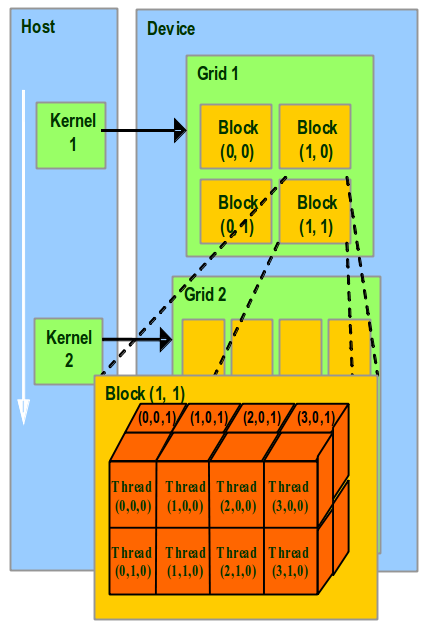
\includegraphics[width=0.35\textwidth]{Images/cudaBlocks.png}
\caption{Task allocation between grids, blocks, and threads in a GPU}
\label{fig:cudaBlocks}
\end{center}
\end{figure}
	
Memory is not shared by the GPU and the CPU. Memory must be copied from the host (CPU) to the device (GPU) when a calculation must be preformed. This memory transfer runs in \O{n} time. Because memory must be copied, certain operations such as matrix subtraction are not well suited to be parallelized. A matrix subtraction on the GPU would take \O{n} time for the memory transfer and \O{n/threads} time for the operation, whereas whereas the same operation on the CPU will take \O{n} time.

Memory on the GPU is divided into global memory, which is accessible from each thread in each block, shared memory, which is accessible from each thread in a given block, but not threads in other blocks, and register memory, which is only accessible from a single thread. The memory diagram for a GPU is shown in Figure \ref{fig:cudaMem}. Registers are accessed faster than shared memory, which is in turn accessed faster than global memory. When data is moved from the CPU to the GPU, it is placed in global memory.

\begin{figure}[h]
\begin{center}
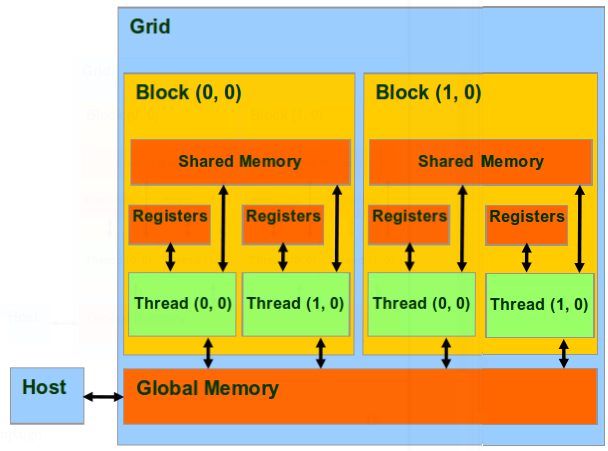
\includegraphics[width=0.35\textwidth]{Images/cudaMem.png}
\caption{The GPU memory hierarchy}
\label{fig:cudaMem}
\end{center}
\end{figure}

\section{User Interface}
%TODO - was my work insignificant?
A significant portion of the development of the editor was spent designing and implementing a graphical user interface (GUI) to display the result of the editing operations performed. The user interface was written in C++ using a cross-platform framework called Qt, available from Nokia under a LGPL open-source license. The use of Qt allowed for rapid GUI development and created a beneficial abstraction of GUI commands into image editing function calls. 

As Qt also contains a multimedia framework, its use simplified the extension of the program to standard image formats; the QImage class provided support for reading .bmp, .gif, .jpg, .png, .pgm, and .tif files from disk, as well as writing .bmp, .jpg, .png, .tif with an optional quality setting. In addition to the standard image formats provided by QImage, custom image (.ppc) and video (.pvc) codecs were created and encoders and decoders implemented. These will be discussed further in a later section.

The GUI is arranged to display the original image on the left and the modified image on the right. The scale of the images can be changed using zoom functions, and the modified image can be reset to the original image without requiring reopening, and thus decoding, the file from disk. This functionality was provided in lieu of undo/redo functionality, which would require either a large amount of memory to be allocated or the creation of inverse functions for all implemented functionality. Videos can be played using a control bar at the bottom that also allows for frame by frame inspection.

Compression is implemented so as to display a new dialog containing both the modified media and the compressed version. This allows for side-by-side comparison of the compression quality achieved as well as comparison among multiple compression levels. The peak signal-to-noise ratio (PSNR) is also reported as a measure of the compression quality chosen. 

\section{Image Editing}
Several common image editing operations were explored and then implemented in the editor. These were then further extended to video editing by applying them to each frame sequentially. Each operation implemented is discussed in detail below.

\subsection{Grayscale}
%TODO - unify ARGB // 0xffRRGGBB
Because the image was stored internally in ARGB format, the conversion to grayscale requires application of the luminance formula to each pixel: \begin{equation*}luminance = 0.3*red + 0.59*green + 0.11*blue \end{equation*}
This is in contrast to an image in YCrCb format, where the color space would simply be thrown away. The luminance result was then clamped to fit into an 8-bit unsigned char (0 $\leq$ value $\leq$ 255) and assigned to all of the red, green, and blue color values. All values resulting from color calculations in all future editing operations can be assumed to be clamped to the same range before being assigned to the resulting image. 

\subsection{Brightness}
Increasing the brightness of an image can be achieved by scaling each of the RGB values by a specified factor. This adjusts the luminance of the entire image.

\subsection{Contrast}
Contrast is a measure of the distance of each pixel from the average luminosity. In order to increase contrast,  a linear combination of the average luminosity and the RGB values are taken:
\begin{equation*} red = (1 - factor)*average\_lum + (factor)*red \end{equation*}

\subsection{Saturation}
In contrast to contrast, increasing saturation requires scaling the RGB values of a pixel away from its luminosity, rather than the global average luminosity. The formula appears the same as for contrast, with $average\_lum$ replaced with $lum$.

\subsection{Crop}
Cropping was implemented to remove unwanted portions or highlight desired portions of an image. The function takes four parameters defining the top-left and bottom-right corners of the desired sub-image.

\subsection{Rotation}
Rotation was implemented using both Gaussian sampling and nearest-neighbor sampling of the original image in order to determine pixel color values in the rotated image. If the image rotation is a multiple of 90$^\circ$, nearest-neighbor sampling is used to generate a one-to-one matching, while Gaussian rotation is used otherwise. The Gaussian used was defined with variance 0.6 and radius 4 pixels. 

\subsection{Scale}
Scaling was also implemented using Gaussian sampling, also with variance 0.6, but with a radius that linearly depends on the scaling factor to compensate for the enlarged (or shrunken) size of the image.

\subsection{Blur}
Blurring was performed using a 3x3 convolution filter that weights the original pixel heavily, but allows for contributions from neighboring pixels:
{\small{
\begin{equation*}
mask[3][3] = \left\{ \left\{\frac{1}{16}, \frac{2}{16}, \frac{1}{16}\right\}, \left\{\frac{2}{16}, \frac{4}{16}, \frac{2}{16}\right\}, \left\{\frac{1}{16}, \frac{2}{16}, \frac{1}{16}\right\} \right\}
\end{equation*}
}}

\subsection{Edge Detection}
Edge detection was similarly implemented as a 3x3 matrix convolution, but with a mask that highlights pixels with colors sufficiently different from its neighbors:
\begin{equation*}
mask[3][3] = \left\{ \left\{-1, -1, -1\right\}, \left\{-1, 8, -1\right\}, \left\{-1, -1, -1\right\} \right\}
\end{equation*}

\section{Compression}
The two compression algorithms that were implemented both sequentially and in parallel were the biorthogonal 9/7 discrete wavelet transform (DWT) with a dead-zone quantizer for images and a closed-loop DPCM quantizer with motion estimation for videos.

\subsection{Image Compression}

%TODO - DWT diagram?
The particular implementation of the DWT that was used was the lifting implementation. This implementation is the same one used in the JPEG2000 standard. The forward transform (FWT) works on an array of real values. The values are filtered into low and high frequency sub-bands, which are each downsampled by a factor of two. This is done with two prediction filters and two update filters. A prediction filter sums each odd index with a scalar multiple ($\lambda$) of the sum of its neighbors, while an update filter does the same, but for even indices. The coefficients used were $\lambda_{predict0}$ = -1.586134342, $\lambda_{update0}$ = -0.05298011854, $\lambda_{predict1}$ = 0.8829110762, and $\lambda_{update1}$ = 0.4435068522. The result is an array of the same length, with the high pass sub-band retained in the odd indices of the array and the low pass sub-band is retained in the even indices of the array.

This sparse representation of the image is then passed through the dead-zone quantizer. The dead-zone is given by the user in the form of a percentage of coefficents which should be quantized to zero. The program then estimates the actual dead-zone size using a piecewise continuous function constructed with experimental data.

The inverse transform (IWT) is preformed using the same computational structure as the FWT, but with the filters in reverse order and using the negatives of their coefficients.

A sketch of the parallel algorithm for image transformation is as follows. First, the image is transferred into GPU memory. The different color components must be transformed separately, so the 32 bit 0xffRRGGBB image data is rearranged such that all the red, blue, and green values are in continuous memory. This is done in one parallel step, where each thread moves one color value, and is not done in-place. Each row of each continuous color region is then transformed in parallel. Due to the iterative nature of the FWT, the algorithm cannot be preformed in one step. Once each row is transformed, each continuous color region is transposed separately. The FWT is then applied to each row (previously column) of each continuous color region in parallel. This completes the one level 2D FWT. Another transpose, FWT, transpose, and FWT is applied to perform the two level 2D FWT.

The parallel IWT is simply the same process with filter order reversed and negated coefficients. The IWT must also rearrange the continuous color regions back into 32 bit 0xffRRGGBB format.

\subsection{Video Compression}

%TODO - DPCM diagram?
A closed-loop DPCM uniform quantizer with 8x8 pixel block motion estimation was implemented for video compression. A sketch of the algorithm is as follows. For the first frame, the previous frame is set to all zeros. The encoded previous frame is subtracted from the current frame, $d[n]$, which is then quantized and inverse quantized, $\hat{d}[n]$. This value is summed with the encoded previous frame, $\hat{x}[n-1]$ and set as the new encoded previous frame for the next iteration, $\hat{x}[n]$. Motion vectors are then found for each 8x8 block which minimize $\sum$$\mid$$x[n]$ - $\hat{x}[n-1]$$\mid$, where $\hat{x}[n-1]$ is shifted by the motion vector, and the quantized result along with the motion vectors are sent to the communication channel for encoding.

Decoding is simpler than encoding and involves simply summing the previous decoded frame, $\hat{x}[n-1]$, shifted by the motion vectors, with the inverse quantized incoming frame, $\hat{d}[n]$.

The parallelization comes into play with the search for optimal motion vectors. As previously stated, simple operations such as matrix addition or subtraction do not offer significant speedup when preformed on the GPU. An exhaustive search for motion vectors lends itself well to parallelization, however. Each block on the GPU is assigned one 8x8 block of pixels and is given the current and previous frames. Each thread within that block is assigned one motion vector, and calculates the sum of the absolute values of the differences between the pixels within the current and previous block, shifted by the motion vector. From this pool of all potential motion vectors, a parallel reduction is preformed, reducing the time to find the minimum value in an array from \O{n} in a serial implementation to \O{log(n)} in parallel. The first iteration of the reduction compares n/2 sets of 2 elements, and returns the smallest of each. The next iteration then compares n/4 sets of 2 elements, and returns the smallest of each. This continues until the smallest element is found. In this case, the motion vector with the smallest mean absolute difference is found and returned. An example can be seen graphically in Figure \ref{fig:reduction}.

\begin{figure}[htbp]
\begin{center}
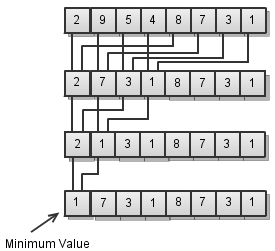
\includegraphics[width=0.35\textwidth]{Images/reduction.png}
\caption{Reduction algorithm in a GPU}
\label{fig:reduction}
\end{center}
\end{figure}

Sample code which came with the CUDA SDK was modified and used for both the reduction and the transpose. A second set of non-parallelized algorithms are also supplied to compare with GPU accelerated algorithms, and for users who do not have a compatible GPU.

\section{Encoding}
In addition to the standard image formats provided by Qt's QImage class and decoders implemented for .qcif and .cif formats, custom image and video codecs were created and encoders and decoders for them implemented. They are the parallel picture codec (.ppc) and parallel video codec (.pvc), respectively. The encoder works similarly for both image and video, running the media through the appropriate compression algorithm using the percent compression provided by the user in a dialog box, applying the specified lossless encoding combination, and outputting the resulting byte stream. A file header is output specifying the media's width and height, the compression applied, the encoding modes applied, the total number of bytes in the stream, and the number of frames in the case of video. Decoding simply applies the appropriate decoders and generates a new QImage from the resulting bytes.

\subsection{Huffman}
Huffman coding is one of the most common lossless compression techniques. It is a variable-length coding system derived from the Shannon-Fano code, and published in 1953. It has the property that no code-word is the prefix of another, allowing for rapid decoding while receiving communication. The algorithm achieves this by building a tree of symbols from the least probable at the leaves to the most probable at the root, and assigning codes based on the path traveled in the tree to reach the symbol. Thus, more frequent symbols have smaller code-words. Using this technique, Huffman coding achieves optimal entropy when the symbol probabilities are powers of two, and very close to optimal entropy otherwise. Huffman coding is used today in JPEG, MPEG, and MP3.

%TODO - just curious, whats the lookup time on std::map?
The algorithm implemented in this editor generates the codes using the tree and then stores them in a std::map, allowing for rapid lookup of the code-word corresponding to the symbol, rather than searching the whole tree (256 symbols). The decoding process re-creates the table and repeatedly adds a bit to the code-word and determines if it is valid, beginning a new code-word when a match is found. The std::map structure was also used for this lookup, in anticipation of quick hashing and thus lookup, but it is possible that a tree-traversing implementation could outperform the current implementation, based on the disappointing runtime results of the decoding algorithm, as discussed in the results section and seen in Table \ref{table:decode_times}.

\subsection{Run-Length}
Run-length compression is the conceptually easiest compression encoding to implement. It replaces a long string of identical symbols, a run, with two symbols indicating the symbol and the length of the run. It is especially effective when used in conjunction with another form of compression that tends to generate large numbers of insignificant symbols, such as the DWT compression scheme implemented in this editor. Each run encoded was limited to 277 symbols due to the numerical limits of the unsigned char data type. Runs of one or two symbols were not encoded so as not to increase the number of bytes.

\subsection{Arithmetic}
Arithmetic encoding is a process that represents a fixed-length sequence of symbols with a particular value that both the encoder and decoder can understand. It is, in a sense, a means of hashing the stream to be encoded. The underlying principle is the use of the probabilities of symbol occurrences to generate a value [0,1) that can be represented as a binary fraction and transmitted over the communication channel. It tends to approach entropy, and is well-suited for real-time decoding. It does, however, suffer from fixed-precision problems, as discovered in our implementation and discussed in the results section below.

\section{Results}

\subsection{Image and Video Editing}
%TODO - do we want to mention this? Each number in this section is the average of twenty runs. 
On the GPU edge-detection was performed on ``world.jpg" (1024x1024 pixels) in an average of 153.9 ms. The same operation on the CPU took 372.9 ms on average, for a speedup of 2.42 times. These results can also be representative of the blurring operation, as both operations perform a 3x3 pixel convolution, just with a different mask.

On the GPU, ``world.jpg" was turned to grey in 53.45 ms. The same operation on the CPU took 102.85 ms, for a resulting speedup of 1.92 times. This speedup is also representative of the contrast, saturate, and brighten operations, as they are all per-pixel operations.

Rotate, crop, and scale had no analogous GPU functions implemented with which to compare performance. 

Video editing was preformed frame-wise, so the speedups would be the same as for the still image cases.

\subsection{Image Compression}
%TODO - do we want to mention this? Each number in this section is the average of twenty runs. 
The test system used for image compression metrics was a custom built 2.66GHz Core 2 Duo PC running Windows 7 with 4GB of available RAM and an NVIDIA GeForce 8800GTS with 640MB of available VRAM. On the GPU, ``lena.jpg" (512x512 pixels) was transformed and inverse transformed in 136.95 ms on average. The same pair of transforms on the CPU averaged 374.95 ms. The resulting speedup was 2.74 times. On the GPU, ``monarch.jpg" (768x512 pixels) was transformed and inverse transformed in 198.1 ms. The same transforms on the CPU took 557.35 ms, for a speedup of 2.81 times.

As seen in Figure \ref{fig:lena_psnr}, the program was able to maintain a relatively high PSNR of about 30 dB while zeroing out up to 95 percent of the coefficients. The transform and inverse transform are not lossless, as even if the deadzone of the quantizer does not exist, it still rounds coefficients to integer values.

\begin{figure}[htbp]
\begin{center}
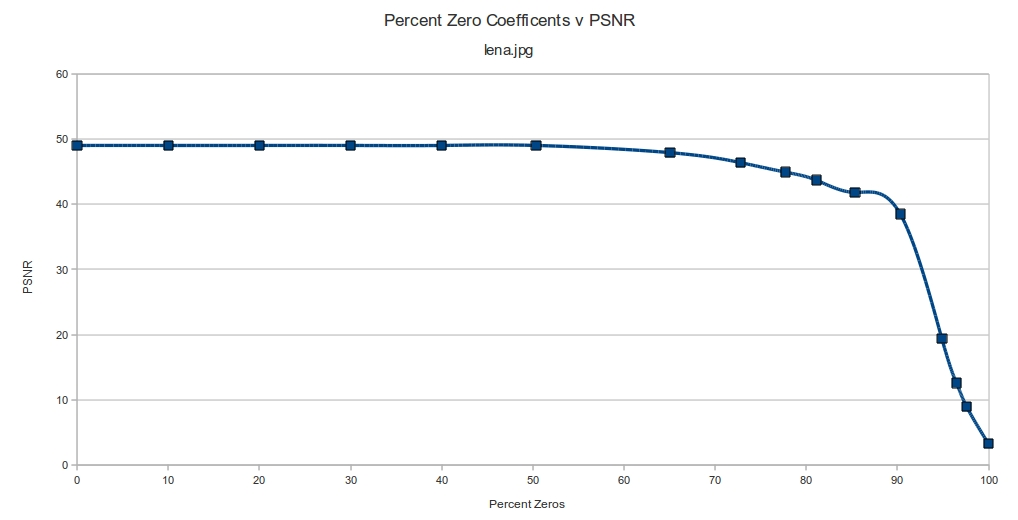
\includegraphics[width=0.5\textwidth]{Images/lena_psnr_chart.jpg}
\caption{PSNR results, ``Lena.jpg"}
\label{fig:lena_psnr}
\end{center}
\end{figure}

%TODO - add this picture?
%\begin{figure}[htbp]
%\begin{center}
%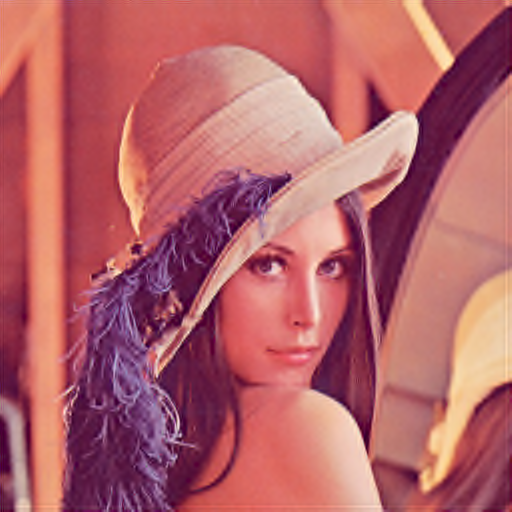
\includegraphics[width=0.5\textwidth]{Images/lena_93_337158_pct_zeros.png}
%\caption{93\% Coefficients Quantized to Zero, ``Lena.jpg"}
%\label{fig:lena_93}
%\end{center}
%\end{figure}

\subsection{Video Compression}
%Each number in this section is the average of twenty runs.
The test system used for video compression metrics was the same system used for image compression metrics. ``Glasgow100.qcif" and ``bus.cif" were used to test video encoding speed. ``Glasgow100.qcif" contains 100 frames of 176x144 video, while ``bus.cif" contains 150 frames of 352x288 video.

On the GPU, ``glasgow100.qcif" was encoded in 3.465 seconds on average. On the CPU, ``glasgow100.qcif" was encoded in 34.275 seconds. The resulting speedup was 9.89 times. On the GPU, ``bus.cif" was encoded in 21.304 seconds. On the CPU, ``bus.cif" was encoded in 206.443 seconds. The resulting speedup was 9.69 times.

As seen in Figure \ref{fig:glasgow_psnr}, the program was able to maintain a PSNR of over 30 dB when it had more than approximately 100 quantization levels. Interestingly, there are spikes of very high quality video for quantization levels which are powers of two. The PSNR when there were 512 quantization levels was infinite, meaning that compression was lossless.

\begin{figure}[htbp]
\begin{center}
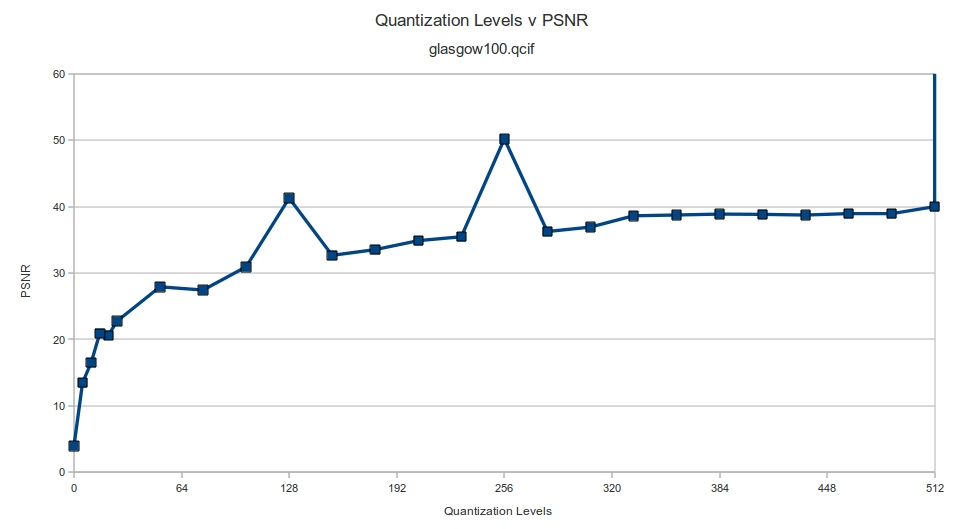
\includegraphics[width=0.5\textwidth]{Images/glasgow100_psnr.jpg}
\caption{PSNR results, ``glasgow100.qcif"}
\label{fig:glasgow_psnr}
\end{center}
\end{figure}

%TODO - Add amount of VRAM
\subsection{Encoding}
``Lena.tif" (512x512 pixels, 787 KB) was used as a test image on a 2.4 GHz Core 2 Duo MacBook Pro with 2 GB of available RAM and an NVIDIA GeForce 8600M GT. Encoding was performed using all eight possible encoding permutations at multiple compression ratios (0\%, 50\%, and 90\%), all using GPU acceleration. At all three compression levels, all three encoding methods combined still completed with a maximum runtime time of 1.53 seconds. Runtimes for decoding were generally significantly higher, as can be seen in Table \ref{table:decode_times}. Performing run-length decoding was insignificantly more costly than performing no decoding, and both methods were significantly more efficient than the other encoding methods. Times were similar for all three compression levels, as expected.

\begin{table}[htdp]
\caption{.ppc decoding runtimes}
\vskip -15pt
\label{table:decode_times}
\small{
\begin{center}
\begin{tabular}{|r|c|}
\hline
 & Runtime (s) \\
 \hline
 \textbf{None} & \textbf{0.726}\\
 \hline
 Huffman & 7.126\\
 \hline
 \textbf{Run-Length} & \textbf{0.749}\\
 \hline
 Arithmetic & 8.318\\
 \hline
 Arith. over Huff. & 10.544\\
 \hline
 Huff. over Run & 6.648\\
 \hline
 Arith. over Run & 6.851\\
 \hline
 Arith. over Huff. over Run & 9.897\\
 \hline
\end{tabular}
\end{center}
}
\end{table}

The .ppc file sizes generated at all three compression ratios and under all encoding permutations can be seen in Table \ref{table:filesize}. While it would be expected to be the case that a combination of all three encoding methods would produce the smallest file size, it is not the case. This can be blamed on the implementation of arithmetic encoding, which consistently doubles the file size when used, as it encodes four symbols (1-byte unsigned chars) in a double (8-bytes). This is because the implementation used does not include scaling and thus runs out of precision early in its execution when a large number of symbols (256) is used. Of all the single-option methods, Huffman compression generates the smallest file size, even including the symbol lookup table, but this is improved by first using run-length encoding to reduce the number of symbols to encode. As this method has an acceptable decoding runtime as well, this could be implemented as the default .ppc encoding method.

\begin{table}[htdp]
\caption{Filesize by encoding technique and compression percentage}
\vskip -15pt
\label{table:filesize}
\small{
\begin{center}
\begin{tabular}{|r|c|c|c|}
\hline
 & 0\%  & 50\% & 90\% \\
 \hline
 None & 2.1 MB & 2.1 MB & 2.1 MB\\
 \hline
 Huffman & 872 KB & 827 KB & 389 KB\\
 \hline
 Run-Length & 1.7 MB & 1.5 MB & 311 KB\\
 \hline
 Arithmetic & 4.2 MB & 4.2 MB & 4.2 MB\\
 \hline
 Arith. over Huff. & 1.7 MB & 1.7 MB & 774 KB\\
 \hline
 \textbf{Huff. over Run} & \textbf{831 KB} & \textbf{786 KB} & \textbf{152 KB}\\
 \hline
 Arith. over Run & 3.3 MB & 3 MB & 681 KB\\
 \hline
 Arith. over Huff. over Run & 1.7 MB & 1.6 MB & 299 KB\\
 \hline
\end{tabular}
\end{center}
}
\end{table}

% TODO - Add video encoding/decoding runtimes and filesizes for a sample video

\section{Conclusions}
For ``glasgow100.qcif", each compressed frame was calculated in 34.6544 ms using the GPU-accelerated algorithm. This equates to encoding 28.85 frames per second, indicating that the editor can preform the exhaustive search for the optimal mean absolute difference motion vectors in real time. Each frame in ``bus.cif" was encoded in 142.02 ms on the GPU, for 7.04 frames per second. For a video of this size, real time motion estimation cannot not achieved using the current algorithm.

Due to slight arithmetic differences, the GPU and the CPU did not always find the same vectors. In motion-ambiguous regions, like the sky in the beginning of the Glasgow sequence, there was some variation between the two sets of motion vectors.
%TODO - motion vector images?

Speedups were noticed for both image operations and image compression, but were not as significant as the video speedups. As stated earlier, per-pixel operations are not expected to receive large speedups from parallelization. The time it takes for image compression could be further reduced by breaking the image into tiles and using shared memory on the GPU, but this would lead to tiling artifacts, one of the things the DWT is supposed to get rid of.

Speedups could also be achieved by removing all alpha value bytes from the program, as they increased memory usage by 25\%, increasing the bottleneck of copying memory to and from GPU. This would also improve the speed of file encoding and compression, and reduce the resulting file sizes on disk.

On both of the test systems, the GPU was simultaneously driving the system's display. This signifigantly reduced the amount of available VRAM. Neither system was able to preform image editing operations on a 4096x4096 image. This could be alleviated by processing the images in tiles, or obtaining a secondary GPU for dedicated computations.

%TODO - Conclusions about encoding processes?

%\nocite{*}
\bibliographystyle{IEEEbib}
\bibliography{Multimedia}

\end{document}
